\chapter{Technical Design}

This chapter will give a overview of the structure of the application as well as some choices taken when developing the research product, Nevrolens. 

\subsection*{Unity Scene Graph}

Within Unity a \textit{Scene} consists of a \textit{scene graph} which is a tree structure of \texttt{GameObjects}. By default a scene consist of a \texttt{Directional Light} lighting up the scene at its default light source and a \texttt{Main Camera} which is the view point of the running game. In addition, the MRTK library will add two objects to the scene graph, one called \texttt{MixedRealityToolkit} which contains configuration of the Mixed Reality features and systems. This is where input systems are defined and where control of spatial awareness and boundary detection is handled, in short all features and sensors of the HoloLens system or other AR system are defined and controlled here. The other object added by MRTK is the \texttt{MixedRealityPlayspace}, this encapsulates the \texttt{Main Camera}, but is lacking any useful documentation on what its purpose is. The name could be hinting at it being the parent of the \textit{Playspace}, meaning all \texttt{GameObjects} in the game. However, even MRTK demos seem to ignore this object and thus it has not been used in this project either.

The functionality of the scene graph, other than organizing GameObjects, is that child objects inherit the position, rotation and scale of their parents, thus simplifying transformation of complex object. This naturally structures many systems, however in a AR application there can be many independent 3D objects floating in space. In addition, some objects are dependent not on their parent, but on a defined object \texttt{Transform}. Therefore, some organization is needed and some objects are placed by choice and convenience rather than any practical reason. Another practical use for child objects are the use of the \texttt{GameObject.GetComponentsInChildren()} and \texttt{GameObject.GetComponentInParent()} methods which allows for simple access to \texttt{Components} in child and parent \texttt{GameObjects}, this is however of limited use as such dependencies in code has a tendency to result in tedious bugs.

The top most application specific object of the project is the \texttt{BrainSystem}, this acts as the parent GameObject for all objects defined by the application. The right side of \autoref{fig:brainsystem} gives an overview of all 3D object in the \texttt{BrainSystem}. The \texttt{InfoBoard} on the right, the button group, or \texttt{HandMenu} in the center and the complete brain model with axes etc. named \texttt{GameWorldSpace}, are spatially independent systems all having \texttt{BrainSystem} as a parent, this can also be seen in \autoref{fig:brainsystem} in the scene hierarchy on the left side. The reasoning for having the parent object \texttt{BrainSystem} is purely to to tidy up the top layer of the scene graph and having a clear distinction of project specific custom objects. 

The main attraction within the \texttt{BrainSystem} is the \texttt{GameWorldSpace}, it is the parent of the brain model and all objects with are spatially dependent on the brain. This allows for movement and scaling of the whole model worldspace. This is also the local space of the synchronized multiplayer world. 

% notice that the blue "black board" on the right, the button group and the brain are independent spatially.

\begin{figure}[ht]
    \centering
    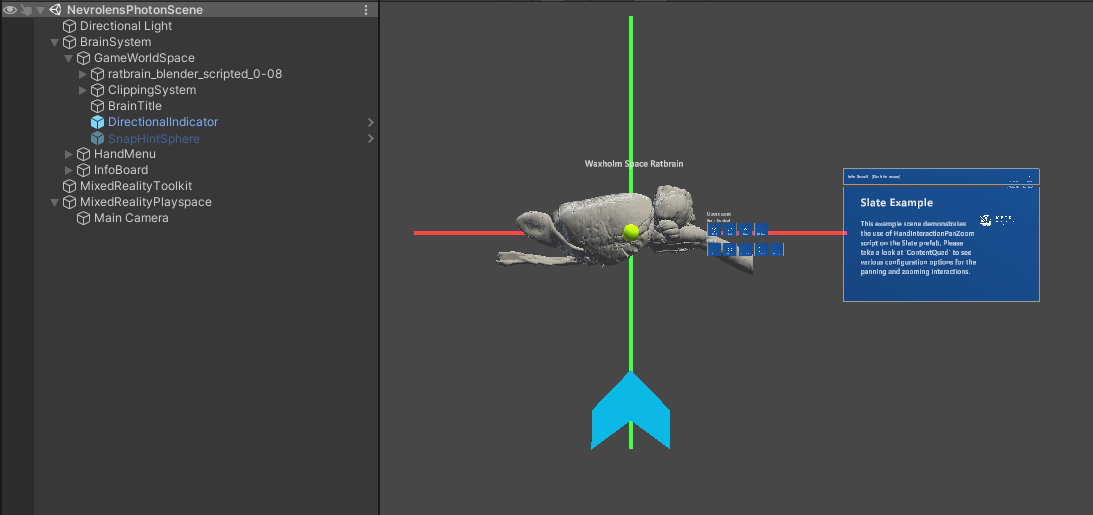
\includegraphics[width=\textwidth]{fig/brainsystemoverview5.png}
    \caption{Every 3D object in the \texttt{BrainSystem}}
    \label{fig:brainsystem}
\end{figure}
% In general there is few limitations on how to structure the scene graph, its functionality other than structural,
\subsection*{Networking Solution}

Multiplayer games in Unity can be created in numerous ways, in the development phase of this project three solutions were explored; UNET,  LiteNetLib and Photon PUN2 . Common for all are that they are mature, reliable and are well documented, they all support multiple device types including all devices within the scope of this project, there are however some very clear differences making the choice for this project quite simple.
% mlapi, mirror, playfab
UNET is Unity's own default networking solution, it provides high level functionality and is generally easy to use. It is however deprecated and will be discontinued by the end of 2021, an open source fork of the networking API, called \textit{Mirror} has seen continuing development and improvement, but because of the state of the original project, both were deemed nonideal. Unity is working on a new networking solution called \textit{MLAPI}, it is in alpha stages but shows great promise.

LiteNetLib is a open source, and more low level framework. It is intended for use cases where in-depth control of the networking processer are wanted or needed, if high performance and low latency is important this would be a good choice. It supports peer-to-peer and self-managed servers. Because this project can be thought of a small scale proof of concept, it is of limited concern whether the networking is highly performant and seeing as a low level API is more complicated to implement it is neither a optimal use of a single developers time.

Lastly, Photon PUN2 is the an high level networking library with managed hosting and a free basic plan for up till 20 concurrent users. This makes it ideal for small projects and single developers. It is also the general first choice for networking solution in Unity and its surge in popularity was a reason for Unity abondonign 


% mature, reliable and easy to use with 

